Rancangan variabel kepentingan akan dilakukan dengan menggunakan metode Random Forest. Metode Random Forest akan menghasilkan variabel kepentingan yang dapat dilihat pada Gambar \ref{fig:variabel-kepentingan}. Variabel kepentingan ini akan digunakan untuk melakukan analisis risiko autentikasi.
Berikut adalah rancangan variabel kepentingan yang akan digunakan untuk melakukan analisis risiko autentikasi.
\begin{figure}[H]
    \centering
    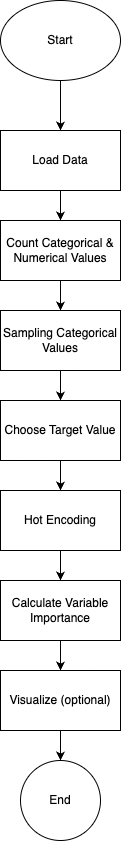
\includegraphics[width=0.2\textwidth]{BAB_TESIS/IMAGES/vim.drawio.png}
    \caption{Rancangan Variabel Kepentingan}
    \label{fig:variabel-kepentingan}
\end{figure}

Gambar \ref{fig:variabel-kepentingan} menjelaskan bahwa variabel kepentingan akan digunakan untuk melakukan analisis risiko autentikasi. Variabel kepentingan ini akan digunakan sebagai input untuk melakukan analisis risiko autentikasi.
Setelah data berhasil di-import akan diakukan penghitungan kategorikal dan numerikal data. 